% *************************************************************************
\chapter[Computational Enzyme Engineering: Activity Screening using Quantum Chemistry.]
{Computational Enzyme Engineering: Activity Screening using Quantum Chemistry.\label{ch1}}
\chapauth{Martin R. Hediger$^{a}$
\chapaff{$^{a}$Z\"urich\\
m---@---.ch}}
% *************************************************************************


% *************************************************************************
% *************************************************************************
\section{Abstract}\label{sec:abstract}
\begin{itemize}
\item QM Screening of CALB and BCX
\item Screening 317 single and 111 double mutants with av. 29 h per barrier and 1 CPU per interpolation point
\item Correct mechanisms using PM6
\item Barriers in agreement (calc. 18.5, exp. 17.0 kcal/mol)
\item 15/22 correctly predicted (using many approximations and not full model)
\item No bias, more active double mutants identified
\item largely automated
\item For CALB lowest barriers close to WT, BCX lowest barriers lower than WT
\end{itemize}
% *************************************************************************


% *************************************************************************
% *************************************************************************
\clearpage
\section{Motivation}\label{sec:mot}
Let us imagine two companies $a$ and $b$.
Both companies use very similar technical equipment to carry out the biotechnological process $\ce{X}$ $\xrightarrow{Biocatalyst}$ $\ce{Y}$ using two different versions of a biocatalyst.
Company $a$ uses an enzyme with a rate constant $k_{a} = 1000s^{-1}$ while company $b$ uses an enzyme with $k_{b} = 2000s^{-1}$.
Letting all other things be equal, the process of company $b$ will therefore only require half the time to produce one Mole of product compared to the time required for company $a$.
Company $b$ therefore can save energy required to keep the reaction volume at a certain temperature.
The need for efficient catalysts arises from such an outline and the commercial implications of these considerations are immediate.\footnote{In this work, we use the terms \textit{enzme} and \textit{bio-}/\textit{catalyst} interchangeably.}\\
Increasing the performance of enzymes however is still far from trivial and forms a growing body of research.
What is clear though is that the development of such catalysts is costly, in terms of manpower, material and energy -- if carried out in the laboratory.
A number of companies have in fact formed around this demand: Novozymes (DK), Genzyme (US) or DSM (NL) to name but a few\cite{meyer2013use, kirk2002industrial, beilen2002enzyme, schmid2002use}.\\
Laboratory costs can however be saved to a large part if the development is carried out \textit{in silico}.
The proof that computational results are as reliable as experimental results has been provided not too long ago\cite{claeyssens2006high}.
The foundation for successful application of computational enzyme engineering has thus been laid out.
It is therefore natural to ask: Why hasn't this become more important yet?
Why are there not more job openings at pharmaceutical and biotechnology companies looking for computational enzyme engineers?
The field, after all, did receive the Nobel price in Chemistry in 2013.
As a side note, computational modeling of aero- and fluid dynamics, semiconductor properties, pharmaconkinetics/pharmacodynamics or civil engineering is well beyond the point of having to justify itself as of strategic relevance.\\
More important questions asked and answered in this review:
\begin{itemize}
\item Is it possible to screen for mutant activity using quantum chemical methods?
\item Which quantum chemical model can reproduce the accepted mechanism?
\item What are the time requirements depending on the model size?
\item How should the program be configured?
\item What modeling procedure/sequence is needed? Which tools are useful?
\end{itemize}
By giving an overview and some details in this article, I hope to, at least in part, answer the above questions.\\
\textcolor{red}{[ARE THE QUESTIONS ANSWERED?]}
% *************************************************************************


% *************************************************************************
\clearpage
\section{Introduction}\label{sec:intro}
In this review, we aim to provide an introduction into the topic of modeling of enzyme catalysis for people from both within or from outside the field, with emphasis on aspects of activity screening and some emphasis on commercial applicability.
We outline the latest achievements, methods in use and required developments to further establish computational enzyme engineering and screening also in commercial practice.\\
While the process engineering team in company $a$ from above is working on improving reaction conditions, consider the enzyme engineer required to engineer the currently used catalyst to match (and possibly outperform) the activity of the catalyst used by company $b$.
Following the hypothesis that the function of an enzyme depends on its structure, in order to change the function, some kind of change to the structure has to be introduced and this in general requires the introduction of one or more mutations of amino acids in the primary structure of the enzyme.
However, as is well known in the community, it is almost impossible to predict, how a mutated variant of an enzyme will behave[\textcolor{red}{REFS?}, Bornscheuer?].
Will it at all be possible to express it and will it even fold and if so, will it be more or less active and specific relative to the wild type?
Are its pH properties still the same and is it of similar temperature stability?
Even the most reasonably suggested mutations (except for elimination of the catalytic residues) will not allow to predict \textit{qualitatively} with confidence if the mutated enzyme will be more or less active.
Therefore it appears as if the only reasonable strategy were to carry out systematic screening studies.\footnote{By \textit{screening} we mean the construction of a large library of mutants which are inspected and compared for a specific property like activity.}
As was pointed out initially, such studies are expensive in the laboratory and therefore an alternative is to carry them out on the computer.
The aim of such initial computational screening is not to provide high-accuracy kinetic data but much rather to provide a reliable, qualitative activity estimate of a preferably large mutant library.
It is important to note that while the initial computational screening might be of limited accuracy, its major value is the provision of a systematically developed library of mutants.
Based on the screening, promising candidates can then be pipelined into a more demanding computational method for further characterization.

\noindent\textcolor{red}{[Physical property of interest:]}\\
Ideally the physical property of interest guides the selection of the appropriate computational method and not the other way around, therefore a brief overview on computational methods is provided.
The method has to be adapted to the physical property of interest\\
- Thermal and structural integrity\\
- pH dependent activity\cite{ludwiczek2013strategies}\\
- Active site hydration\\
- Binding, \textit{c.f.} drug design where the target protein is constant\\
- \textcolor{red}{Binding effects not considered}\\
- Catalysis: \textit{C.f.} biofuel production or synthesis applications where the substrate is mostly non-variable.

\noindent\textcolor{red}{[Different modeling objectives:]}\\
1) One Enzyme -- Multiple Substrates:
These tasks are usually addressed by docking approaches and studies involving millions of substrates have been published\cite{zhou2010high}.\\
2) Multiple Enzymes -- One Substrate:
The approaches to this task, as it appears, are much less established.
Why is that?
A number of factors can be of influence among which are that modeling of different variants of an enzyme will also mean to differentiate between multiple (possibly coupled) protonation states which is non-trivial.
Furthermore, modeling of reactivity always involves modeling of a transition state, which is non-trivial and for which there is no standard fail safe approach.

\noindent\textcolor{red}{[Application context:]}\\
- Academic: screening can assist in generation of new hypothesis about structure/function relationships\\
- Commercial: commercial application is restricted by time-to-delivery of predictions, accuracy/reliability, screening spectrum and convenience of use.
Notefully, in a commercial context, accuracy can be of less value than reliable qualitative prediction of relative activities.

\noindent\textcolor{red}{[Review structure and audience:]}\\
This review is written for a general audience.
For specialized details, the reader is referred to the primary literature.
Since molecular modeling of enzymes has been reviewed extensively over the recent years, we do not attempt to provide all fundamentals of the subject.
Instead, we focus on screening aspects of computational enzyme engineering.
The intention is to provide an accessible introduction into the field of quantum chemical modeling of enzymatic reactions, highlight advantages of using quantum chemistry and also point out situations where special care needs to be taken.\\
By 2014, quantum chemical methods have been in use to study enzymatic reactions for around three decades.
What is new however is that quantum chemical methods can now be used also in \textit{in silico} screening assays of enzymatic activity and this is also part of the focus of this review.\\
\textcolor{red}{Applications.}
We will discuss application of the approach to the modeling of two enzymes: CALB and BCX.
% *************************************************************************




% *************************************************************************
% *************************************************************************
\clearpage
\section{Methods}\label{sec:methods}

\subsection{Calculation Engines}\label{sec:calculation_engines}
The focus of this article is on the application of quantum chemistry for the screening of enzyme mutants.
So instead of attempting to incompletely review modern computational chemistry methods, only a few selected facts relevant for the following are highlighted.
Details are found in text books on the subject\cite{young2004computational, jensen2007introduction, cramer2013essentials}.\\
Most fundamentaly, computational descriptions of a molecular system are done using either (parametric) \textit{force fields} or \textit{ab initio} electronic structure methods.\footnote{\textit{Molecular mechanics}, \textit{empirical } or \textit{classical mechanics} are other expressions for force field methods.}
Force field methods are useful in studying structural behavior of enzymes over a significant time period (approaching the millisecond scale) and can provide details about structural rearrangement of an enzyme.\\
Chemical reactivity however is accompanied by changes in the electronic structure of the system which require quantum chemical methods to be described.
For the sake of the argument, semi-empirical, density functional and \textit{ab initio} methods are all understood to form the set of quantum chemical methods.\\
\textbf{Quantum Chemical Methods.}
Quantum chemical methods attempt at solving the Schr{\"o}dinger equation for the molecule, the solution of this equation will yield the wave function of the system.
However, depending on the specifics of the quantum chemical method, the solutions are different.
Now, since every quantum chemical method provides its own description of the wave function (or electron density in density functional methods) and all properties, such as energy or charge distribution, are \textit{derived} from the wave function (or the electron density), it is essential to note that every method has \textit{its} own chemistry depending to the wave function (or density) it produces.
As a consequence, hydrogen bonding patterns of a structure can be different when optimized with two different quantum chemical methods.
Therefore, it is good practice to verify the predictions of one quantum chemical method against, perhaps, higher-level methods, or to at least ensure that the obtained conclusions are consistent with the method against which results are compared.
With regard to the modeling of enzymatic reactions, if a method can reproduce the generally accepted mechanism then there is a good chance that at least qualitatively reliable conclusions can be made using this method.\\
In the applications, the semi-empirical PM6 method\cite{stewart2007optimization, stewart2009application} was used together with the MOZYME technology\cite{stewart1996application}\footnote{\textit{Semi-empirical } essentially means that the calculation consists of a parametrized and unparametrized component which results in efficiency gains.}.
In a comparative study, PM6 is found to provide results approaching density functional accuracy\cite{schenker2011assessment}.
Furthermore, calculations on small active site models of the two enzymes allow to reproduce the generally accepted mechanisms.
The MOZYME technology allows to localize the molecular orbitals obtained during the self-consistent field calculation which results in computational demands scaling linearly with system size.
Additionally, the implementation of the PM6 method is actively being developed further to take into account properties such as dispersion or solvation\cite{rezac2009semiempirical, vrezavc2011halogen}.
In essence, these two technologies in combination therefore provide the accuracy and efficiency required for modeling of enzymatic reactivity in a screening assay.

\subsection{Molecular Modeling}\label{sec:modeling}
A variety of molecular modeling approaches is available in the literature, all suitable for different applications.
We briefly outline two of them and then introduce in more detail the approach used in the screening studies of the application section.\\
\textbf{Cluster approach.}
Among the most popular are the so called cluster models, where a larger or smaller part of the enzyme active site is extracted into a separate model and then all calculations are carried out on this smaller model.
Structural integrity of the model is preserved by applying constraints on the truncation points and among the most prominent applications of this approach is the kinetic discrimination between possible competing mechanistic alternatives\cite{noodleman2004quantum, himo2006quantum, siegbahn2009recent}.
This technique, in principle, can be used in enzyme activity screening studies, however care has to be taken that no mutations are introduced into the model which can only be accommodated because of the reduced model size, \textit{i.e. } because there appears to be space for a side chain where in reality there would not be any.\\
\textbf{Full Enzyme Models.}
Using a full model of the enzyme structure prevents such ambiguity, but raises a number of issues as well.
Including the full enzyme structure in the calculation naturally increases the computational demands significantly.
Thus when running calculations on a full enzyme structure, careful consideration of the the trade-off between accuracy and efficiency becomes very important.
One way of addressing this issue is by using so called hybrid method which combine a quantum chemical and a classical mechanics based calculation.
The advantage of these methods is that they are capable of producing highly accurate results, the setup of such calculations is however still not as straightforward as is required for large scale screening approaches.
An alternative is to describe the complete system using the same, albeit lower level of theory (\textit{i.e. } PM6) which reduces efforts to setup the calculation significantly.
This is the approach of the applications described below.\\
As was outlined above, semi-empirical methods in combination with linear scaling technologies, which are readily available in a number of programs (GAMESS, MOPAC and others), are sufficiently efficient and allow for some degree of programmatic customization, which is of great relevance for later data analysis.\\
\textbf{Calculation of Reaction Barrier.}
Irrespective of the method used, calculating the activation energy requires to estimate the difference between the transition state and the most stable state of the system before the transition state on the reaction coordinate.
This is a non-trivial problem and no generally applicable methods exist to do this, solving this problem will therefore always at one point require direct input from the modeler.
Furthermore, characterization and identification of a transition state is computationally very demanding operation and, especially in large systems, is likely to fail.
A reasonable approach is therefore to approximate the transition state by linearly interpolating the structure along the reaction coordinate of the rate determining step of the total reaction.
If carried out carefully, this approach can provide very good approximations to transition state.\\
\textbf{Linear Interpolation.}
In both applications outlined below, the basic procedure to obtain a reaction barrier consists of preparing structures for the enzyme substrate complex (``ES'') and the first intermediate (CALB: ``TI''\footnote{Tetrahedral intermediate}, BCX: ``GE''\footnote{\label{foot:ge}Glycosyl enzyme}) and calculating the reaction barrier between for the ES$_\text{CALB}$-TI and ES$_\text{BCX}$-GE pairs, respectively.
For these two pairs, the reaction barrier is calculated by preparing a set of 10 intermediate structures which approximate the structure of the system along the reaction coordinate, Fig. \ref{fig:calb_reaction}A.\footnote{In the literature, the terms \textit{interpolation}, \textit{linear transit scan}, \textit{reaction coordinate calculation } or \textit{adiabatic mapping} are frequently used to indicate essentially the same kind of procedure.}
\begin{figure}[htbp] 
\centering
\begin{minipage}{0.49\linewidth}
A
\end{minipage}
\begin{minipage}{0.49\linewidth}
B
\end{minipage}
\begin{minipage}{0.49\linewidth}
\includegraphics[width=1.00\linewidth]{calb-interpolation-1.png}
\end{minipage}
\begin{minipage}{0.49\linewidth}
\includegraphics[width=1.00\linewidth]{0000-wt.eps}
\end{minipage}
\caption{
\textbf{A:} Illustration of linear interpolation.
It is visible how the substrate and the nucleophilic oxygen of S105 approach each other.
Also visible is the proton transfer to H224 in the late interpolation frames and how the oxyanion hole (T42) follows the increasingly negative carbonyl oxygen of the substrate.
\textbf{B:} Evaluation of the system energy for each interpolation frame results in an approximate reaction barrier (calculation done with PM6).
}
\label{fig:calb_reaction}
\end{figure}
As a side note, it is mentioned that extending this interpolation approach to the complete set of screened mutants requires some development effort and depends on the software used.\\
By evaluating the energies for each interpolation frame for the two reactions ES$_\text{CALB}\rightarrow$TI or ES$_\text{BCX}\rightarrow$GE, an approximate potential energy surface of the reaction is obtained, Fig. \ref{fig:calb_reaction}B.
The quality of the results of this approach are strongly dependent on how careful the modeling of each of these structures is carried out.
Since the geometry of every interpolation frame is optimized individually, it is possible that adjecent interpolation frames optimize into significantly different local minima, this is a frequent reason for meaningless results.
It is therefore advisable that the two end points of the interpolation are not to different in structure.\\
After using the same approach to calculate activation energies of the mutants, low activation energies correspond to high anticipated activity of the variant and so candidates for further characterization can be identified.\\
It is noted that in this approach, the focus is on the catalysis and it is assumed that binding of the substrate by different mutants is similar, an observation which is also made in experiments\cite{ludwiczek2013strategies}.\\
\textbf{Requirements.}
The most basic requirements are that a structure representing a bound intermediate along the reaction pathway is available.
For the modeling it is advantageous to have a bound intermediate which can then be modified into the substrate, preserving its natural binding pose.
Alternatively, a homology model could be used.
Using a single model as the template for both the intermediate of the reaction, as well as the preceeding stationary point is another advantage because the structural differences between these structures will be small and will less likely lead to non-conclusive reaction barriers in the interpolation.
Furthermore, ideally the mechanism for the rate determining step is established in the literature.
In case no generally accepted mechanism is reported, a preceeding study in a small model structure could analyse kinetically competing mechanistic alternatives.\\
\textbf{Preparation of Mutant Structures.}
The structure of the mutants can be prepared with any kind of molecular modeling software, however it is advantageous if the software can be controlled programmatically.
One important note is made.
It is frequently observed that specific pairs of mutants can not be accommodated in the same model because the two new side chains would clash.
In order to facilitate the approach, these variants are discarded from the screen.
Furthermore, side chain orientations can be oriented in various ways and are defaulted using a crude local optimization procedure which is builtin into PYMOL.
Ionization states of side chains greatly complicate the screening and the best approach most likely is to consider different ionization states only at a later stage of the assay.

\subsection{Software}\label{sec:software}
The largest part of the calculations in the applications below have been carried out with the MOPAC software\cite{stewart1990mopac}.
This software is designed to be convenient to use and efficiently to setup.
It offers various semi-empirical calculation engines and linear scaling techniques and is optimized towards working with PDB formatted data structures.\\
To prepare the molecular models, it appears that PYMOL offers a huge range of functions and can be controlled programmatically, which is critical for the preparation of a large, systematic set of mutants.
It has to be noted, that still molecular modeling and computational screening consists of a lot of customization work, especially for data analysis the output format of the various programs is not very suitable.
This might also be contributing to preventing quantum chemical methods from becoming more popular in industrial environments.
Docking methods for example are implemented in software which is designed towards user friendlyness and have established themselves in industry.
Another project is GTKDynamo which looks very promising, but which sofar however is supported only by a small community\cite{bachega2013gtkdynamo}.
% *************************************************************************




% *************************************************************************
% *************************************************************************
\clearpage
\section{Applications}\label{sec:apps}

\subsection{Overview}\label{sec:overview}
From a technical point of view, a computational screening assay is characterized by its computational efficiency, \textit{i.e. } how long it takes for the calculations to complete, its user friendlyness, its accuracy and the modeling prerequisites.
In the following, two applications of the presented screening method are introduced.
It is shown how the method performs relative to these mentioned criteria.

\subsection{Engineering {\textit{Candida antarctica} Lipase B}}
\textbf{Relevance and Summary.}
Using CALB as a test case, we develop an efficient modeling protocol, verify the calculations with experimental results and show how quantum chemical methods can be used for enzyme activity screening\cite{10.1371/journal.pone.0049849, hediger2013silico}.
The reaction studied is the hydrolysis of $N$-benzyl-2-chloroacetamide.\\
CALB has been highly characterized over the years such that its structure, physical properties and expression systems are well documented\cite{uppenberg1994sequence, uppenberg1995crystallographic}.
The enzyme is a highly established catalyst with applications in organic synthesis, formulation technology\cite{gayot2003modification} and in kinetic resolution of racemic mixtures\cite{gotor2006candida, naik2010lipases, chaput2012contribution}.
Furthermore, since the enzyme is known for its reactive promiscuity\cite{bornscheuer2004catalytic, CBIC:CBIC200800318}, it provides an ideal development platform for applications for which existing biocatalysts are only of limited efficiency.
One such application is the hydrolysis of amide bond containing lipophilic compounds.
While in principle amide bonds can be cleaved by proteases or peptidases, these enzymes are found to be less active towards hydrophobic substrates such as amide containing lipids\cite{nakagawa2007engineering}.
Therefore, engineering CALB activity towards ${\text{CO}-\text{NH}}$ bond containing hydrophobic substrates would greatly expand its applicability.\\
\textbf{Structure and Mechanism.}
Briefly, the active site in CALB consists of a catalytic triad (S105, D189 and H224) and an associated oxyanion hole.
The mechanism is understood to follow the generally accepted mechanism of serine protease active sites\cite{hedstrom2002serine}, Fig. \ref{fig:calb-mechanism}.
\begin{figure}[htbp] 
\includegraphics[width=0.98\linewidth]{calb-mechanism.eps}
\caption{
Reaction scheme for the formation of the tetrahedral intermediate in CALB.
In this work, R$_1$: -CH$_2$-Cl, R$_2$: -CH$_2$-C$_5$H$_6$\cite{hediger2013silico}.
}
\label{fig:calb-mechanism}
\end{figure}
The rate determining step is believed to be the nucleophilic attack by O$^\gamma$ of S105 on the carbonyl carbon C$^{20}$ of the substrate.\\
\textbf{Calculations, Experimental Verification and Calibration.}
After establishing a working proof-of-concept of the screening approach using a limited set of three mutants\cite{10.1371/journal.pone.0049849}, the method was scaled up to screen a set of 386 mutants of the CALB active site\cite{hediger2013silico}.
This set consisted of single- to eight-fold mutants and of these, the activity of 22 mutants was measured experimentally.\\
The accuracy of the method was calibrated in terms of qualitative predictivity, \textit{i.e.} how likely can the method predict if a mutant will have higher or lower activity than the wild type.
For this calibration, the following issues need to be addressed.
In the experiments, the activity relative to the WT, in principle, ranges from zero to infinity.
In the calculations on the other hand, the activity of a mutant is determined by the difference between the mutant reaction barrier and the wild type barrier\footnote{If a mutant has a lower reaction barrier than the WT, it is understood to have higher activity.}.
However, even for a very active mutant, the reaction barrier is not expected to be zero and so in this approach, since lower barriers are related to higher activities, the amount by which a mutant can be more active than the wild type is in principle limited.
Conversely, since the reaction barrier of a mutant can in principle be arbitrarily high, the amount by which a mutant could be less active than the wild type might be infinite.
Establishing a direct quantitative relationship between differences in reaction barrier heights and relative experimental activities is therefore not very meaningful.
Instead, it is more meaningful to only qualitatively compare activities, \textit{i.e.} if a mutant has higher or lower activity than the WT (both experimentally and calculated), and use these results for determining the predictivity.\\
To cluster the results into increased/decreased activities it is therefore necessary to decide above/below which activity a mutant is considered being part of either the higher-activity or lower-activity clusters.
Considering the relatively narrow spread of experimental activities\footnote{The experimental improvement factors range from 0 to roughly 11 times wild type activity.}, mutants with $\geq1.2$ times the wild type activity are considered improving while mutants with $<0.8$ times the wild type activity are considered degrading (mutants inbetween are considered as neither improving nor degrading)\cite{hediger2013silico}.
The computational results are clustered in a similar way.
A cutoff value for the calculated reaction barriers is introduced \textit{below} which the mutant is considered improving and above which the mutant is considered degrading.
It is found that at a specific cutoff value (12.5 kcal/mol), the method qualitatively predicts activity of 15 out of 22 mutants correctly, Fig. \ref{fig:diag-predictivity}.
\begin{figure}[htbp] 
\includegraphics[width=1.00\linewidth]{diag-predictivity-truncated.pdf}
\caption{
Agreement between predicted and experimental qualitative activity relative to wild type\cite{hediger2013silico}.
}
\label{fig:diag-predictivity}
\end{figure}
Noteworthy, mutants with both higher as well as lower activity are correctly predicted.
Importantly, the advantage of clustering the mutants in this way is not apparent maximum agreement with the experimental data in the first place, but much rather to provide a lower limit for the predictivity under the given set of approximations.
It is important to keep in mind that it will be unlikely to have calibration data available in a computational enzyme activity assay, since idealy it is performed \textit{before} wet-lab experiments are started.
Therefore, such an approach is further justified since at the initial outset of a screening study, the focus is mostly on narrowing down possible candidates from a large library, \textit{i.e. } the focus is on obtaining qualitative conclusions rather than quantitative results\cite{agresti2010ultrahigh}-- this is the true value of computational screening.
Following such a screening analysis, out of the mutants predicted to have higher activity, a set consisting of as many mutants as can be further characterized is selected and suggested for further study, either computationally or experimentally.\\
\textbf{Screening Results and Discussion of Mutants.}
Identification of mutants with reaction barriers significantly lower than the wild type is found to be difficult.
In the set of 386 screened mutants, we identified only three mutants with a barrier lower than the wild type (a double, a triple and a four-fold mutant) while a large proportion of the mutants has barriers in the range from 12 to 14 kcal/mol.
%\begin{figure}[htbp] 
%\textbf{A}
%\includegraphics[width=0.95\linewidth]{barriers.pdf}
%\caption{
%Reaction barriers of 278 CALB mutants below 19 kcal/mol and after removal of mutants with inconclusive reaction barrier shape\cite{hediger2013silico}.
%}
%\label{fig:reaction-barriers}
%\end{figure}
We find that a large number of mutants need to be screened to identify the best few candidates for further study.
This conclusion is likely even more true in studies where the enzyme is either intrinsically of only very little activity towards a specific substrate (``it does not work'') or where the enzyme already has reached very high activity towards a specific substrate\cite{agresti2010ultrahigh}.\\
Further analysis of the screening results was focused on two residues: W104 and I189.
These are selected because mutations of these positions can provide more space for the substrate which is hypothesized to lead to increased activity, Fig. \ref{fig:calb-views}.
\begin{figure}[htbp] 
\textbf{A}
\includegraphics[width=0.95\linewidth]{calb-active-site.png}
\caption{
CALB active site, some residues omitted for clarity.
SUB labels the substrate.
}
\label{fig:calb-views}
\end{figure}
As seen, W104 and I189 are in direct proximity to the substrate.
From the single mutant data, it is found that the mutants W104Q or W104Y have barriers just around the cutoff value of 12.5 kcal/mol.
However, when in combination with other mutations, such as G39A-W104F-A141Q-I189A (8.3 kcal/mol) or G39A-T103G-W104Y-A141N (9.8 kcal/mol), these mutations are among the most active ones found.
It is noted that it would be very difficult to arrive at these combinations by pure rational considerations of the active site.\\
Analysis of mutations of I189, Fig. \ref{fig:i189g}, provides additional intersting insight into the non-linear effects of various mutations.
\begin{figure}[htbp] 
\includegraphics[width=0.95\linewidth]{011-diag_eval_scre_setL-i189.pdf}
\caption{
Screening of position 189.
Each data point corresponds to a mutant with calculated reaction barrier on the $x$-axis and number of mutations indicated by the value of the $y$-axis.
The data point symbols indicate either of the point mutations I189A/G/H/N or Y.
Data points labeled as ``Other'' do not contain a mutation of I189.
\textit{E.g.} the far left purple square on row 3 indicates a mutant containing I189Y and two other mutations which are not indicated in the graph.
}
\label{fig:i189g}
\end{figure}
Five different mutations of this position are screened but to illustrate the point, the focus is on I189G.
As a single mutant, I189G is found to be completely unproductive (18.9 kcal/mol, far right red triangle in the row ``Mutation Order = 1'' of Fig. \ref{fig:i189g}).
In combination with another mutation (not shown), the barrier is reduced in one case to around 17.5 kcal/mol and in G39A-A141Q-I189G-L278A, the I189G mutation is among the top three mutants found (6.3 kcal/mol).
Conversely, the mutant G39A-A141Q-L278A has a moderately low barrier (10.9 kcal/mol).
These results emphasize the fact that the activity modulating effect of specific point mutations can behave strongly non-linearly and non-additive and should be kept in mind when considering which mutations to include in further studies.
Put differently, these findings illustrate that it is difficult to predict the activity of combination mutants based on single mutant data alone.
Furthermore, since single mutant data is apparently not sufficient to predict combination mutant activity, screening a wide library of mutants should form an essential initial part of any enzyme engineering project.
It thus becomes clear that computational activity screening can provide a major contribution to cost and material use reduction of the total enzyme engineering efforts.\\
\textcolor{red}{\textbf{[Conclusions and Outlook.]}}
In the study presented in the next section, the method is improved with respect to a number of points.
Among these is the fact that not the complete enzyme structure was used in the calculations, due to reasons of exceeding computational effort, instead only amino acids within 8\AA \mbox{ of } the substrate have been included in the model.
The backbone sequence is therefore interrupted, introducing ambiguity in which amino acids to include in the model and in how to orient hydrogen atoms used to complete the valences at the interruption sites and possibly allowing for non-realistic structural rearrangements during the geometry optimizations of the structure.
Secondly, the mutated positions were selected, in part, based on prior knowledge of the enzyme, instead of systematically screening all active site positions.
Lastly, it remained to be shown that the presented approach could also be adapted to mechanistically different reactions of other enzymes.
These points are addressed in the study of the following section.\\
\textcolor{red}{[CONCLUSIONS?]}
Regarding the initially stated criteria against which to compare a computational screening method, it is noted that the method is sufficiently efficient to screen sets of hundreds of mutants, the predictivity is fairly robust however the method could be improved in terms of user-friendlyness.
% -----------------------------------------------------------------

\subsection{Engineering \textit{Bacillus circulans} Xylanase}
\textbf{Relevance and Summary.}
In order to address the points summarized at the end of the previous section, activity of the xylanase of \textit{Bacillus circulans} (BCX) towards an artifical substrate ($ortho$-nitrophenol-$\beta$-xylobioside), Fig. \ref{fig:substrate}, is engineered.
\begin{figure}[htbp] 
\centering
\includegraphics[width=0.85\linewidth]{substrate.pdf}
\caption{
$ortho$-nitrophenol-$\beta$-xylobioside substrate used in BCX study consisting of two xylose units and ONP.
}
\label{fig:substrate}
\end{figure}
Understanding mechanisms of glycoside hydrolases can also be of major relevance to related fields such as biofuel production\cite{ragauskas2006path, yeoman2010thermostable, zhang2011vital, gao2013increased}.\\
\textbf{Structure and Mechanism.}
Due to its use in paper production\cite{bajpai1999application, buchert1994application}, BCX is also well characterized, a number of PDB structures are available and because of its interesting mechanistical features, it is also the subject to ongoing basic experimental research\cite{ludwiczek2013strategies}.
In this study, the mechanism was taken from the literature as reported previously\cite{joshi2000hydrogen,joshi2001dissecting}.\\
In a first step, the wild type (WT) reference reaction barrier is established.
This is a crucial step because all subsequent conclusions about mutants are depending on how good the WT reaction barrier is estimated.
As was done for CALB, only the rate determining step is modeled, Fig. \ref{fig:bcx_mechanism}.
\begin{figure}[htbp] 
\centering
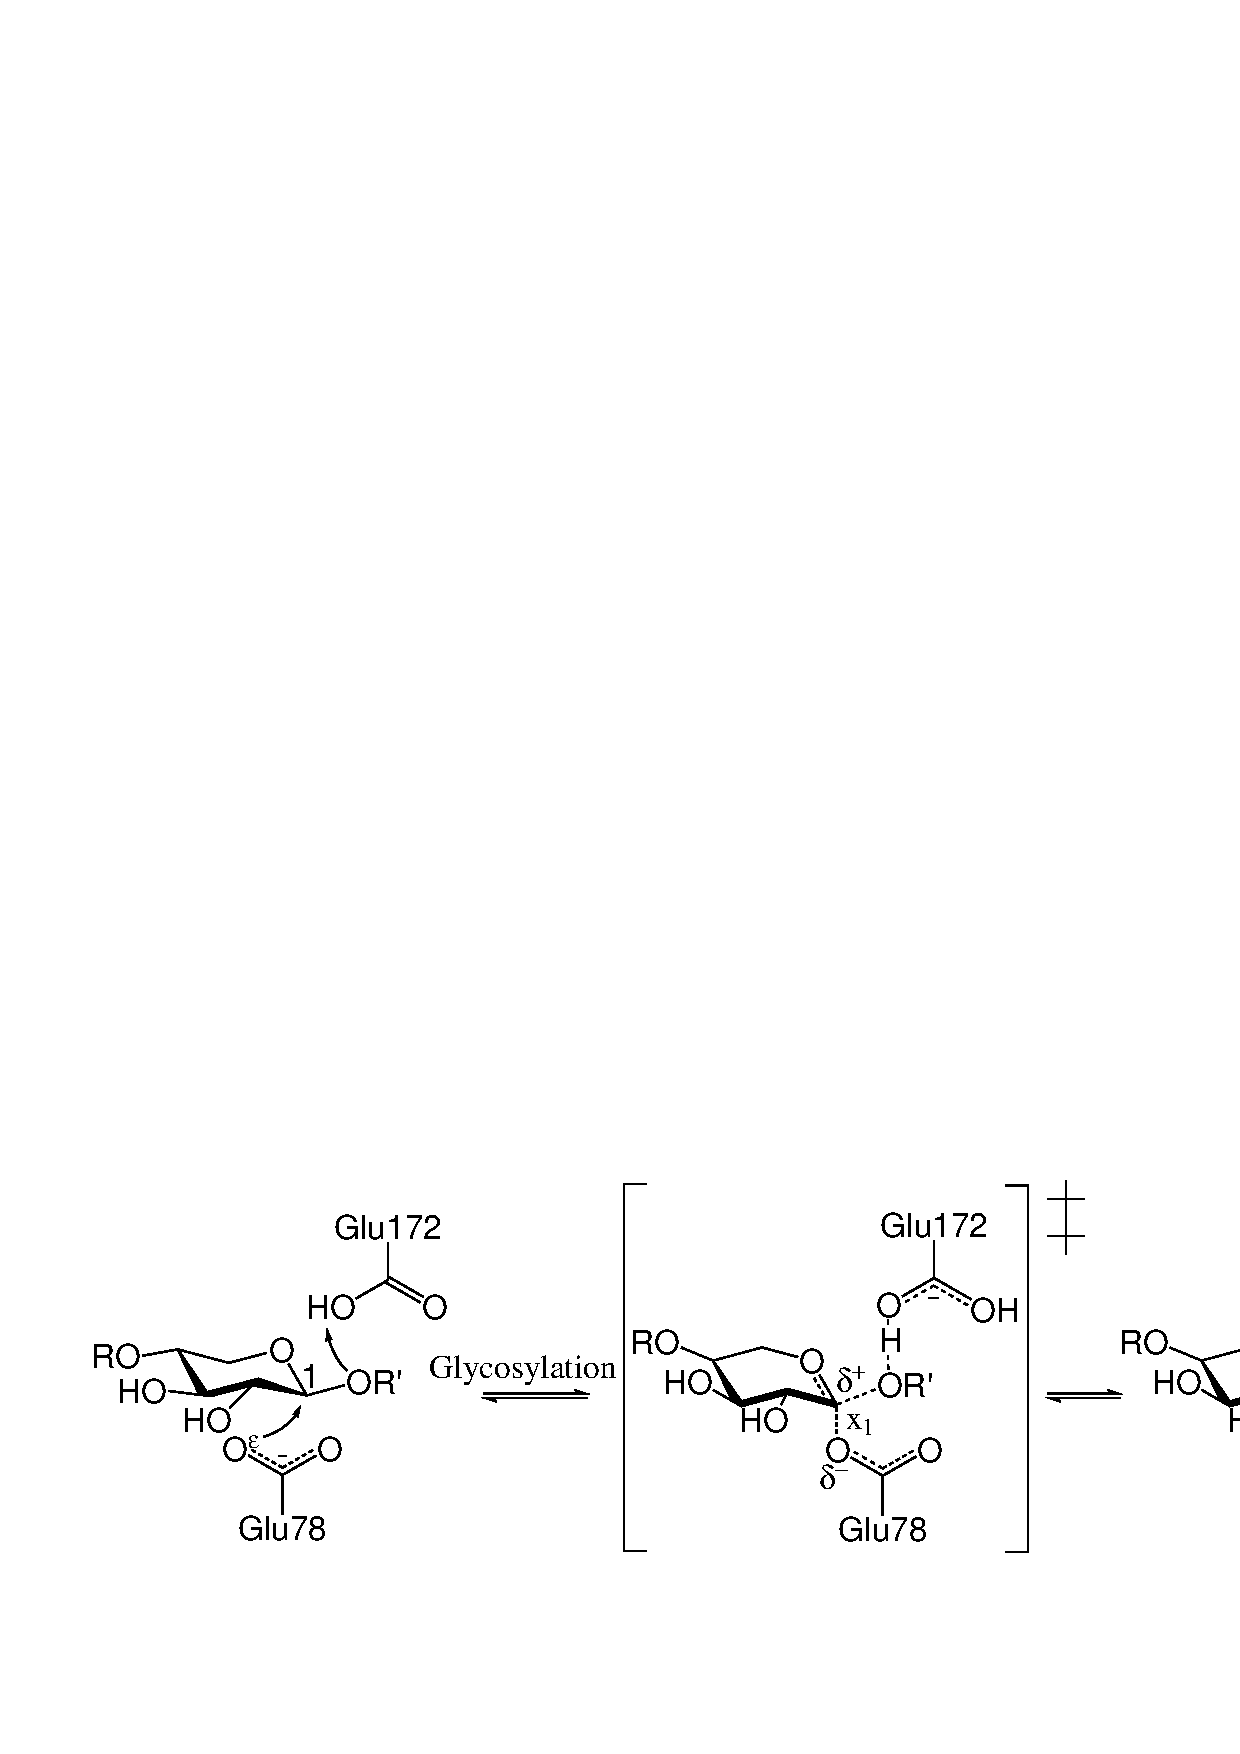
\includegraphics[width=1.0\linewidth]{mechanism.pdf}
\caption{
Rate determining step in conventional glycosylation. $x_1$: constrained reaction coordinate; $R$: xylose; 
$R'$: \textit{ortho}-nitrophenol (ONP).
C$_1$ indicating nucleophilic carbon of first xylose unit\cite{hediger2013computational}.
}
\label{fig:bcx_mechanism}
\end{figure}
Future improvements of the method might consider later reaction steps such as isomerizations or product release.
Noteworthy, in the formation of the covalently linked glycoside-enzyme complex, the substrate isomerises from a chair to a boat conformation.
As outlined in the methods section, the reaction barrier is mapped out by fixing the reaction coordinate ($x_1$ in Fig. \ref{fig:bcx_mechanism}) at discrete, decrementing values while optimizing the rest of the protein structure.
Since the reaction consists of two concerted events (nucleophilic attack by E78 and proton transfer from E172 to ONP), in principle a two-dimensional potential energy surface could be mapped out to determine the reaction barrier.
However, since proton transfer is associated with a rearrangement of the electronic structure, this reaction coordinate is left unconstrained and is handled solely by the quantum chemical method, \textit{i.e.} the proton is free to transfer from or remain on E172.
Forcing the quantum chemical model to do something it would not if left unconstrained most likely results in an increased reaction barrier and therefore it is advisable to keep the number of constraints as low as possible.\\
A PDB structure comprising a covalently linked inhibitor is available (1BVV) and is used as a starting point for the modeling procedure because it gives a very clear indication of how the substrate is located in the active site.
As shown in Fig. 2 in Hediger \textit{et al.} (2013b), two possible modeling pathways were worked out.
In the first one, the ES complex is prepared from the GE structure \textit{before} the GE structure is optimized (see footnote \ref{foot:ge}).
Alternatively, the GE structure is optimized first and then used as a template for the ES structure.
Within this alternative approach, the preparation of the ES structure then just requires minor modifications of substrate conformation before the structure is optimized.\\
Because in this second approach the ES structure very closely resembles the optimized GE structure, it is possible to concentrate the optimization of the ES structure only on the active site, while the remote part of the enzyme remains fixed at the optimized geometry of the GE structure.
This results in very large gains in computational efficiency, which depend on the layer of residues being optimized around the active site.\footnote{The structural constraints are parameters to the calculation program and are prepared programmatically using a PYMOL script. The way the parameters are submitted to the calculation may vary depending on the software used for calculations.}
Fixing, \textit{i.e.} not reoptimizing an already optimized part of the enzyme however also results in slightly increased energy of the ES structure relative to the fully optimized GE structure and so the reaction barriers will be decreased.
This increase (of ES energy relative to GE) results from multiple minor structural strain forming at the interface between the fixed and optimized layers of the structure.
The observations are summarized in Fig. \ref{fig:bcx_constr_constraint_layers}.
% Panel labels have their own minipages to print on same line
\begin{figure}[htbp] 
\centering
\begin{minipage}{0.42\linewidth}
\textbf{A}
\end{minipage}
\begin{minipage}{0.42\linewidth}
\textbf{B}
\end{minipage}
\begin{minipage}{0.47\linewidth}
\includegraphics[width=0.95\linewidth]{bcx-constraint-layers-ray-occlusion-2.png}
\end{minipage}
\begin{minipage}{0.51\linewidth}
\includegraphics[width=1.00\linewidth]{bcx-barriers-constraint-layers.pdf}
\end{minipage}
\caption{
\textbf{A}: Illustration of optimization layers of BCX with bound ONP substrate.
Color coded residue layers have at least one atom within the indicated distance to any atom of the substrate:
\textit{green} 8 \AA, \textit{red} 10 \AA, \textit{purple} 12 \AA, \textit{cyan} 14 \AA.
\textit{Brown} residues remain at their optimized GE geometry, \textit{dark blue} are residues which are screened for active mutations.
The substrate is visible in the center of the dark blue residues.
\textbf{B}: Calculated reaction barriers for different layers of optimized residues (based on Hediger \textit{et al.} (2013b)).
``MOZ.'': Energy evaluated using the MOZYME linear scaling method.
}
\label{fig:bcx_constr_constraint_layers}
\end{figure}
\\
\textbf{Calculations and Experimental Verification.}
Based on this second approach, \textit{i.e.} using the optimized GE structure as the template for the ES structure, and when not applying any constraints (apart from the reaction coordinate $x_1$), the reaction barrier is found to be 18.5 kcal/mol which is in very close agreement to the experimentally reported value of 17.0 kcal/mol obtained from transition state theory\cite{joshi2000hydrogen}.
This strongly supports that the outlined modeling procedure, the configuration of the quantum chemical method and the included/omitted physical effects provide a meaningful model of the enzyme kinetics.
As pointed out above, when applying constraints on remote parts of the structure, this can decrease the reaction barrier because the ES structure is increased in energy relative to the GE reference point (which is set to zero).
However, it is reasonable to assume that this relative increase will be the same for all studied structures and so cancels out once mutants are compared relative to each other.  
Overall, application of constraints to remote parts of the enzyme is necessary to reach the desired calculation efficiency of one reaction barrier per day when running each interpolation step in parallel.
Furthermore, application of constraints has been widely adopted by the community\cite{himo2006quantum,siegbahn2009recent,liao2012comparison,lonsdale2013quantum}.
The time required for optimizing the structures with or without constraints are found to differ by a factor of six (Fig. 4B in Hediger \textit{et al.} (2013b)).\\
\textbf{Screening Results and Discussion of Mutants.}
By a similar approach as the one outline for the modeling of the WT reaction, it is found that different ways of modeling the set of mutants results in significantly different levels of efficiency, both in terms of required manual efforts as well as in computational time requirements.
We refer to the original publication for details\cite{hediger2013computational} but point out that when, similarly as for the WT, the ES structures of the mutants are based on templates of optimized mutant GE structures, again large gains in computational efficiency are possible (see Fig. 7 in Hediger \textit{et al.} (2013b)).\\
Using PYMOL\cite{PyMOLu}, models of all possible single mutants within a given distance of the substrate are prepared (excluding the catalytically active E78 and E172).\footnote{The PYMOL script used for the preparation of the mutants is available at https://github.com/mzhKU/Enzyme-Screening/blob/master/vsc-bcx.py.}
It is noted that in the current implementation of the presented approach, all mutated side chains are in their default ionization state at physiological pH.
Furthermore, in a number of cases it is not possible to introduce a large side chain in a spatially restricted environment, such cases are discarded.
Lastly, instead of using a side chain rotamer library, each mutated side chain is locally optimized (using an empirical builtin PYMOL function) in the environment of the enzyme before being submitted to the quantum calculation.
This approach allowed to screen a set of 317 single mutants, where on average 29 hours are required to complete the calculations of a full reaction barrier using one CPU for each interpolation point.\footnote{All obtained barriers are provided at http://www.scribd.com/doc/133445214/Supp-Mat-Paper-4.}
From this set of single mutants, for every position $i, j, ...$ in the active site, the mutation resulting in the mutant with the lowest barrier $X_i, Y_j, ...$ is identified.
Then, from this set of single mutants $\{K_l\}$, all possible double mutants $(X_i, Y_j)$ are formed.
Analysis of the reaction barriers of the obtained candidates reveals that the set of double mutants on average has lower activation barriers than the set of single mutants.
Furthermore, the lowest barriers are found among the double mutants, Fig. \ref{fig:bcx_barrier_distribution}.
\begin{figure}[htbp] 
\centering
\includegraphics[width=0.95\linewidth]{barrier-distribution.pdf}
\caption{
Barrier distribution of single and double BCX mutants\cite{hediger2013computational}.
The plot is a histogram of reaction barriers, i.e. how many mutants are identified for a given reaction barrier.
}
\label{fig:bcx_barrier_distribution}
\end{figure}
\\
Analysis of the set of mutants indicates that position 127 has strong influence on the activity (9 of 20 best single mutants carry a mutation at that position).
Inspection of the structural arrangement of the Q127W, W9D/E and N35E mutations points to a number of possible explanations of the observed lower barriers.
One observation is highlighted in Fig. \ref{fig:bcx_rationalization}.
\begin{figure}[htbp] 
\centering
%\includegraphics[width=0.99\linewidth]{analyse-charge.png}
\includegraphics[width=0.69\linewidth]{hbonds-es-wt-q127.png}
\caption{
%Rationalization of reaction barriers.
%\textbf{A} Overlay of WT (black carbon spheres) and Q127W side-chain (green).
%\textbf{B} Stabilizing, coulombic interactions between negative W9D/E or N35E (red) with the nucleophilic, partially positively charged C$_1$ of the substrate.
Overlay of Q127W mutant (green spheres) and wild type enzyme substrate complex.
The Q127W mutation preserves structural integrity but prevents hydrogen bond formation to the nucleophilic E78.
The substrate is in black spheres in the upper part of the figure.
Distances in \AA\cite{hediger2013computational}.
}
\label{fig:bcx_rationalization}
\end{figure}
As discussed above, the mechanism is postulated to involve a catalytically active, negatively charged E78 residue as the nucleophile.
If Q127 stabilizes the negative charge by hydrogen bonding, the nucleophilic character of E78 is reduced.
Replacing the potential hydrogen bond donor Q127 with a non-hydrogen bonding substitute that can preserve overall structural integrity with a side chain of similar size, such as Q127W, could result in increased nucleophilicity of E78, Fig. \ref{fig:bcx_rationalization} A.
Furthermore, as illustrated in Fig. \ref{fig:bcx_mechanism}, the transition state involves a partially positive charge on C$_1$ of the substrate.
Negative charges on side chains (such as in W9D/E) could act as stabilizers of this negative charge and increase catalytic activity in doing so, \textit{i.e.} by stabilization of the transition state.
Similaryl, when ionized, N35E could act in stabilizing C$_1$ but when in neutral protonation state, it could be acting as a hydrogen bond donor to the catalytically active E172.
This rationalization of N35 mutations would be related to a recently proposed \textit{reverse protonation} mechanism\cite{joshi2000hydrogen}, which still is the subject of ongoing research.\\
\textcolor{red}{\textbf{[Conclusions and Outlook.]}}
Contrary to the results from the CALB study, we identified numerous mutants with barriers which are considerably lower than the WT barrier.
This fact might be attributed to significantly promoted catalysis by a better fitting of the substrate in the active site.
% *************************************************************************




% *************************************************************************
% *************************************************************************
\clearpage
\section{\textcolor{red}{Conclusions}}\label{sec:conclusions}
The three most significant findings are that firstly, using linear scaling methods and a number of customized software packages it is possible to carry out large scale computational enzyme activity screening studies.
Secondly, single mutant data is not enough to predict combination mutant activities because the activity modulating effects of the point mutations behave non-linearly when in combination with other mutations.
And lastly, using such a screening approach allows not only to identify mutants for further characterization by higher level methods or experimental verification, but also to formulate hypothesis on how the various mutations actually contribute to increased catalysis.
These findings can then be further exploited in future enzyme engineering efforts.
